\newpage
\section{Opis systemu}
\label{sec:opis}

\begin{todo}
W całym rozdziale najpierw dawać plan co chcemy osiągnąć abstrakcyjny, a potem dopiero implementację.
\end{todo}

\subsection{Architektura}
\label{sec:architektura}

Aby spełnić wszystkie postawione powyżej wymagania, zdecydowano podzielić system na kilka osobnych aplikacji, pomiędzy którymi komunikacja jest zrealizowana za pomocą adekwatnych protokołów sieciowych lub plików. Poszczególne moduły oraz połączenia pomiędzy nimi przedstawiono na rysunku \ref{fig:architektura}. Dzięki takiemu rozwiązaniu, można było wykorzystać dostępne oprogramowanie do symulacji dynamiki oraz kompletne oprogramowanie autopilota stosowane na rzeczywistych BSP. Dużą zaletą zastosowania ArduPilot SiTL\cite{soft:sitl} jest format danych w którym przesyłane są informacje o stanie BSP. Ponieważ jest identyczny z komunikacją wysyłaną z rzeczywistego BSP kontrolowanego z wykorzystaniem \emph{firmware} ArduPilot, można wykorzystywać taki sam program do łączenia z symulacją jak i fizycznym BSP w trybie rzeczywistości rozszerzonej (AR).

\begin{figure}[!h]
    \centering 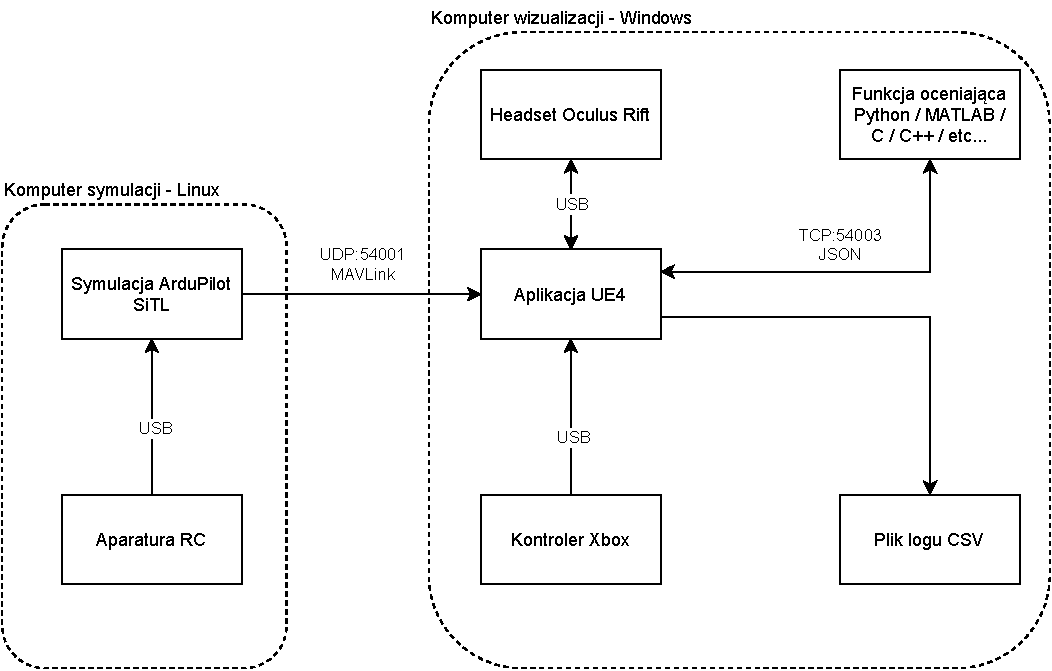
\includegraphics[width=0.8\linewidth]{architektura.pdf}
    \caption{Schemat elementów systemu}
    \label{fig:architektura}
\end{figure}

Aby móc stosować jedną aplikację zarówno z goglami VR oraz AR, wizualizacja została przygotowana z wykorzystaniem Unreal Engine 4\cite{soft:ue4}. To środowisko jest przykładem tzw. ,,silnika'' gier komputerowych. Aby umożliwić uruchamianie tej samej aplikacji na różnych platformach z wykorzystaniem różnego sprzętu, wprowadza liczne warstwy abstrakcji i gotowe klasy, dzięki czemu użytkownik musi jedynie zaimplementować własne kluczowe funkcjonalności programu (tzw. \emph{business logic}). Widoczny na schemacie ,,Kontroler Xbox'' jest popularnym urządzeniem, które wykorzystywane jest w grach komputerowych. Ponieważ także posiada parę dwuosiowych drążków, ale jest prostszy w obsłudze od pełnego nadajnika zdalnego sterowania dla BSP, jest zastosowany jako zastępczy kontroler do prowadzenia prostych testów nowych funkcji bez potrzeby uruchamiania programu symulacyjnego AP~SiTL. Podobnie jak w przypadku urządzeń wyświetlających, sterownik jest zaimplementowany przez zespół Unreal, konieczne było jedynie przypisanie odpowiednich funkcji do przycisków i analogowych osi urządzenia.

Środowisko Unreal Engine oferuje wiele gotowych funkcji, ale przez to jego kod źródłowy jest bardzo obszerny i może być przytłaczający dla nowego użytkownika. Aby umożliwić pisanie funkcji oceniających operatora w językach innych niż C++ oraz rozwiązać wspomniany problem skomplikowania środowiska, ocena operatora także została wydzielona do osobnego procesu.

Wyniki działania wszystkich elementów programu zapisywane są do pliku tekstowego w formacie CSV\cite{rfc4180}. Wadą takiego rozwiązania jest mało efektywne wykorzystanie przestrzeni dyskowej w porównaniu z zapisywaniem liczb bezpośrednio w reprezentacji binarnej. Mimo to zastosowano ten format ponieważ plik danych jest zrozumiały dla człowieka bez stosowania specjalnego dekodera. Ponadto, obsługa plików tego typu jest zaimplementowana w licznych pakietach obliczeniowych m.~in. MATLAB lub Microsoft Excel. Biorąc pod uwagę że symulator ma być elastycznym narzędziem do wykonywania badań, głównym kryterium wyboru było zapewnienie czytelności i swobody wyboru narzędzi dla użytkownika.

\subsection{Aplikacja wizualna}

Jak wspomniano powyżej, cechą charakterystyczną przygotowanej wizualizacji jest wykorzystanie silnika Unreal Engine. Jedną z zalet jest możliwość modyfikowania środowiska do własnych zastosowań, co jest ułatwione przez dostępność kodu źródłowego całego silnika.

\subsubsection{Komunikacja z symulacją BSP}
\label{sec:komunikacja}

Po sformułowaniu wymagań i wstępnym wyborze rozwiązań, w pierwszej kolejności przygotowano prototyp sprawdzający możliwość połączenia oprogramowania ArduPilot z Unreal Engine. W tym celu konieczne było wykorzystanie biblioteki MAVLink\cite{soft:mavlink}, która jest wykorzystywana do komunikacji przez różne systemy BSP, w tym ArduPilot.

Dane o stanie BSP są przesyłane do aplikacji wykorzystując protokół UDP/IP. Został wybrany ponieważ najważniejsze dla działania aplikacji jest otrzymywanie pakietów z minimalnym opóźnieniem. Problem kolejności otrzymywania danych jest rozwiązany przez znacznik czasu znajdujący się w wysłanej wiadomości MAVLink. Utrata pojedynczego pakietu nie jest dużym problemem, natomiast dosłanie brakujących informacji po pewnym czasie jest zbędne, bo mogą już być nieaktualne. Funkcje odczytujące wiadomości MAVLink zostały zaimplementowane w klasie \emph{MavlinkTransformComponent}. Obiekt do którego dołączony jest ten komponent odpowiada za położenie lokalnego układu współrzędnych symulacji ArduPilot w wyświetlanej scenie. Protokół MAVLink wykorzystuje układ współrzędnych lokalnego horyzontu \emph{north-east-down} w metrach. Oś Z tego układu skierowana jest zgodnie z kierunkiem i zwrotem siły ciążenia w locie lub symulacji, oś X prostopadle do niej w kierunku północnym, a Y prostopadle do pozostałych dwóch tak aby utworzyć prawoskrętny układ współrzędnych. Układ globalny oraz lokalne układy współrzędnych w Unreal Engine składają się z osi X skierowanej do przodu obiektu, osi Y prostopadle do niej w prawo, oraz Z do góry obiektu lub sceny, tworząc lewoskrętny układ współrzędnych. Wykorzystywaną jednostką odległości jest \emph{Unreal Unit}, który przy domyśnych ustawieniach jest tożsamy z centymetrami. Konwersja pomiędzy tymi układami współrzędnych jest trywialna, została przedstawiona w formie macierzowej w równaniu \ref{eq:konwersjauklady}.

\begin{align}
    \label{eq:konwersjauklady}
    \mathbf{T}_{n}^{u} & \times \vec{p}_{n} = \vec{p}_{u}
    \\
    \mathbf{T}_{n}^{u} & =
    \begin{bmatrix}
        100 & 0   & 0    \\
        0   & 100 & 0    \\
        0   & 0   & -100
    \end{bmatrix}
\end{align}

Mimo że układ współrzędnych w Unreal Engine jest lewoskrętny, wartości kątów orientacji obiektów są zdefiniowane w tej samej kolejności i o tych samych zwrotach jak w przypadku statków powietrznych. Zakładając zestaw dodatnich kątów orientacji przestrzennej, układ globalny jest przechylany ,,na prawe skrzydło'', pochylany ,,nosem do góry'' i odchylany zgodnie z kierunkiem ruchu wskazówek zegara patrząc od góry, aby otrzymać układ lokalny. Dzięki temu nie jest wymagana żadna konwersja orientacji przestrzennej, jedynie zmiana jej reprezentacji na kwaternion wykorzystując gotową funkcję.

Stosując opisane powyżej konwencje, wiadomości MAVLink \emph{LOCAL\_POSITION\_NED} oraz \emph{ATTITUDE} są interpretowane w kontekście sceny Unreal Engine. Oprócz tego zaimplementowano także obsługę wiadomości \emph{HEARTBEAT}, która zawiera informacje m.~in. o trybie lotu, oraz zgodnie ze specyfikacją protokołu powinna być wykorzystywana do oceny czy połączenie jest aktywne. Korzystając z tych trzech przykładów można łatwo dodać odczyt dodatkowych informacji o stanie statku powietrznego. W pierwszej kolejności należy odnaleźć interesujące dane w liście wiadomości MAVLink obsługiwanej przez system autopilota\cite{soft:mavcommon}, a następnie zaimplementować nowe przypadki w bloku \emph{switch-case} funkcji \emph{UMavlinkTransformComponent::ParseMessage}.

\subsubsection{Interpolacja stanu BSP}
Dane z symulacji są wysyłane z domyślną częstotliwością 25 Hz, ale zmieniając parametry można zwiększyć tę częstotliwość do 40 Hz. Ponadto, z róznych powodów związanych z transmisją przez IP oraz przez radiomodem w przypadku rzeczywistego BSP, zdarza się że niewielka ilość wiadomości nie jest przesłana. Dla zachowania wrażenia płynnego ruchu, które jest szczególnie istotne w przypadku aplikacji rzeczywistości wirtualnej, obraz jest wyświetlany ze stałą częstotliwością 60 Hz. Aby uzyskać odpowiedni stan BSP dla każdej klatki obrazu, konieczne było zastosowanie dodatkowego algorytmu.

W aplikacji wizualnej po otrzymaniu każdej wiadomości z symulacji, aktualizowana jest estymata poprawki czasu symulacji. Aby zmniejszyć wpływ pojedynczych pakietów z dużym opóźnieniem $ T_t $, poprawka $ \Delta t $ pomiędzy czasem liczonym w UE4 oraz czasem AP~SiTL jest aktualizowana tylko o część różnicy pomiędzy nimi. W równaniu \ref{eq:synchronizacja} opisującym tę funkcję parametr $ \alpha $ ma wartość $ 0,2 $, dzięki czemu uzyskano prosty filtr dolnoprzepustowy.

\begin{align}
    \label{eq:synchronizacja}
    \Delta t' &= (1 - \alpha) \cdot \Delta t + \alpha \cdot (t_{UE4} - t_{msg})
\end{align}

Następnie otrzymane wiadomości są zapisywane do bufora, posortowane w kolejności w której zostały wysłane z symulacji. Aby zminimalizować konieczność prowadzenia ekstrapolacji, stany z bufora wyświetlane są z pewnym stałym opóźnieniem $ T_d $, które powinno odpowiadać przynajmniej podwójnej długości odstępu czasu pomiędzy kolejnymi odebranymi wiadomościami $ T_f $. Taka wielkość opóznienia powoduje, że stale można wykonać interpolację pomiędzy dwoma stanami nawet w przypadku utraty jednego pakietu IP. Ta sytuacja została przedstawiona na rysunku \ref{fig:interpolacja}. Prezentowany jest stan interpolacji dla przykładowego parametru $ f(t) $ w czasie $ t_1 $, kiedy pakiet $ p_4 $ nie dotarł poprawnie, ale dzięki opóźnieniu o $ T_d $, $ p_5 $ już jest dostępny.

\begin{figure}[!h]
    \centering 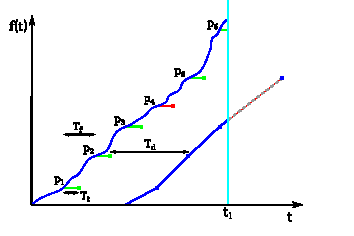
\includegraphics[width=\linewidth]{interpolacja.pdf}
    \caption{Diagram prezentujący algorytm interpolacji}
    \label{fig:interpolacja}
\end{figure}

W momencie rysowania kolejnej klatki obrazu, najpierw obliczany jest moment w czasie symulacji dla którego należy obliczyć stan BSP. Następnie bufor jest przeszukiwany aby znaleźć najbliższy poprzedzający i następujący stan, pomiędzy którymi wykonywana jest interpolacja liniowa położenia i orientacji przestrzennej. W przypadku kiedy nastąpiła utrata większej liczby wiadomości i dostępny jest tylko stan poprzedzający żądany moment, konieczne jest wykonanie ekstrapolacji. Zastosowano ekstrapolację liniową dla pozycji na podstawie ostatniej znanej prędkości liniowej, oraz utrzymanie stałej wartości ostatniej znanej orientacji przestrzennej. Takie rozwiązanie naśladuje stałe wychylenie drążków sterowych dla wielowirnikowca którego układ automatycznego sterowania jest w trybie sterowania pozycją. Bardziej zaawansowane funkcje uwzględniające przyspieszenia liniowe i/lub prędkości kątowe okazały się nieodpowiednie dla obiektu którego regulator dąży do utrzymania stałych parametrów lotu.

\subsubsection{Wygląd symulacji}
Poszczególne zadania do wykonania przez operatora zostały zaimplementowane jako różne ,,poziomy'' lub ,,mapy'' w Unreal Engine. Bez szczegółowej znajomości środowiska można łatwo zmieniać pozycję, orientację i rozmiar widocznych elementów. Referencyjna trasa lotu jest zaimplementowana jako seria stycznych do siebie krzywych Beziera, których punkty kontrolne można przemieszczać w ten sam sposób jak pozostałe obiekty.

\begin{figure}[!h]
    \centering 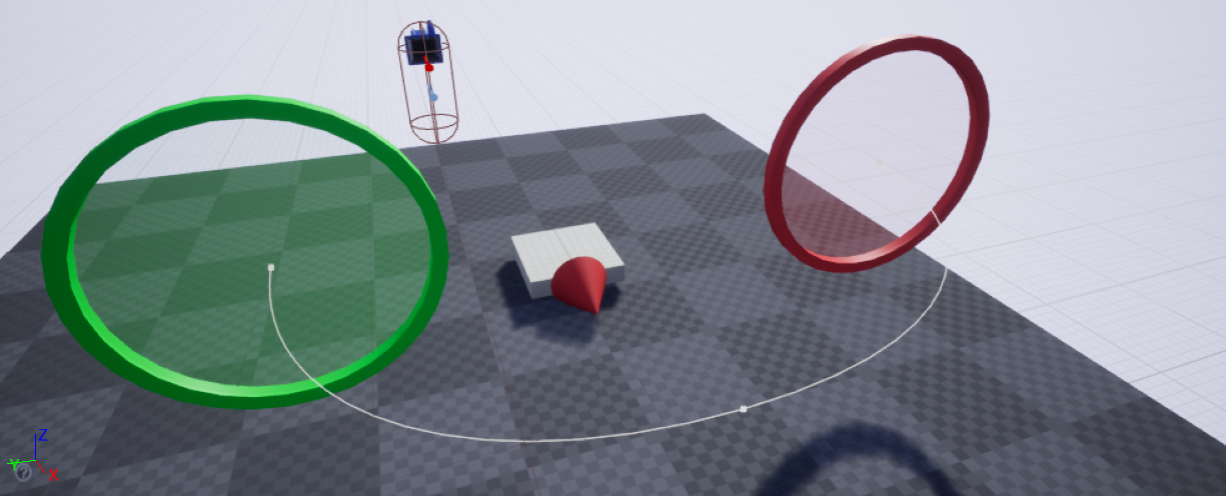
\includegraphics[width=\linewidth]{basicflight.png}
    \caption{Początkowy wygląd aplikacji na etapie testów komunikacji}
    \label{fig:basicflight}
\end{figure}

Przelot przez półprzezroczyste bramki w kształcie kół o promieniu 1~m widoczne na rysunku \ref{fig:slalom}, jest warunkiem rozpoczęcia i poprawnego ukończenia zadania. Przelot przez zieloną bramkę startu rozpoczyna podejście do ćwiczenia, uruchamia pomiar czasu i komunikację z serwerem oceny. Przelot przez czerwoną bramkę końcową kończy próbę pod warunikiem uprzedniego przelecenia przez wszystkie niebieskie bramki kontrolne, jeśli występują. Dla wygody użytkownika przygotowującego zadania, do interfejsu edytora dodano własne przyciski które pozwalają m.~in. na dodanie odpowiednich bramek na końcach trasy referencyjnej oraz automatyczne ustawienie bramek kontrolnych wzdłuż trasy.

\begin{figure}[!h]
    \centering 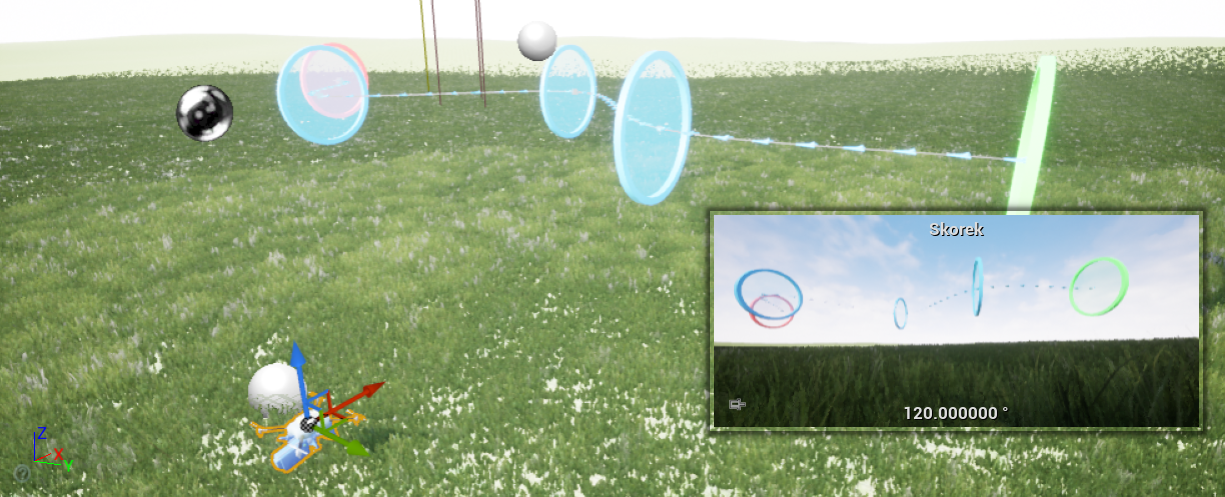
\includegraphics[width=\linewidth]{slalom.png}
    \caption{Zadanie slalom, w prawym dolnym rogu widoczny podgląd kamery FPV}
    \label{fig:slalom}
\end{figure}

Sposób implementacji sterowania BSP pozwala na dodawanie różnych modeli graficznych poprzez rozszerzanie klasy \emph{BaseDrone}. Do tak utworzonego obiektu można dodawać nowe elementy graficzne, dodatkowe zachowania i inne modyfikacje. Użyteczną funkcją po dodaniu nowego modelu jest zmiana położenia kamery do lotu z perspektywy pierwszoosobowej (FPV) w ten sam sposób jak edytuje się środowisko lotu, co przedstawiono na rysunku \ref{fig:edycja-kamery}

\begin{figure}[!h]
    \centering 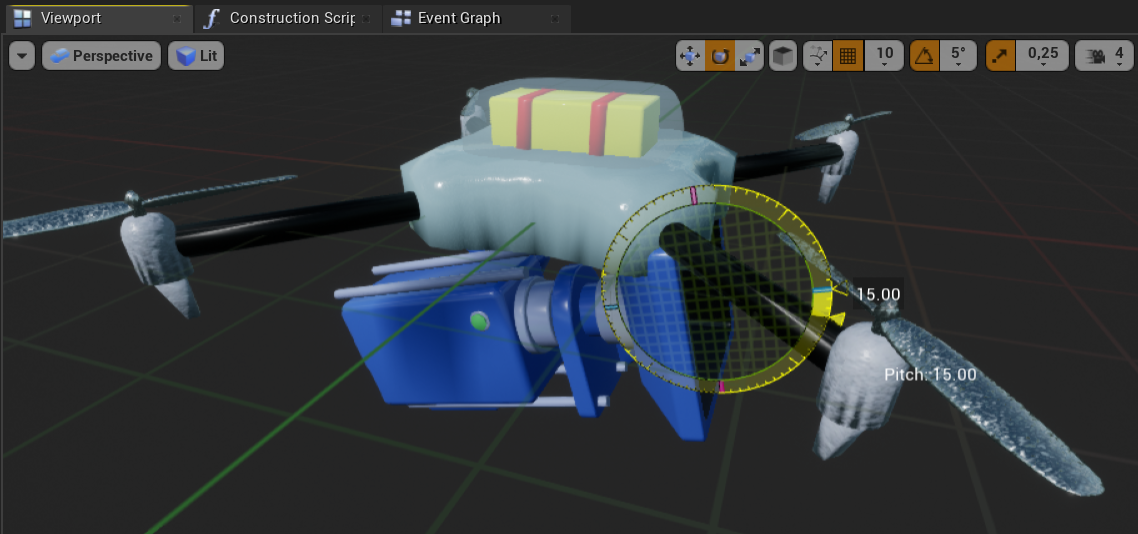
\includegraphics[width=\linewidth]{edycja-kamery.png}
    \caption{Edycja pochylenia kamery zamontowanej na pokładzie BSP}
    \label{fig:edycja-kamery}
\end{figure}

Ponieważ zakłada się stałe zmienianie zadań, aplikacja uruchamiania jest bezpośrednio z programu Unreal Editor. Z tego powodu graficzny interfejs uzytkownika w trakcie działania aplikacji jest ograniczony jedynie do funkcji informacyjnej. Po uruchomieniu aplikacji bez podłączonych okularów wirtualnej rzeczywistości, przy narożnikach okna rysowane są wskaźniki informujące o stanie połączenia z symulacją serwerem oceny, lub o trwającym zapisie danych przedstawione na rysunku \ref{fig:gui-2d}. Aby zachować realizm symulacji i nie rozpraszać operatora nierzeczywistymi obiektami które unoszą się w powietrzu na skraju pola widzenia, te same wskaźniki zostały umieszczone na pulpicie umieszonym bezpośrednio przed operatorem widocznym na rysunku \ref{fig:gui-vr}.

\begin{figure}[!h]
    \centering 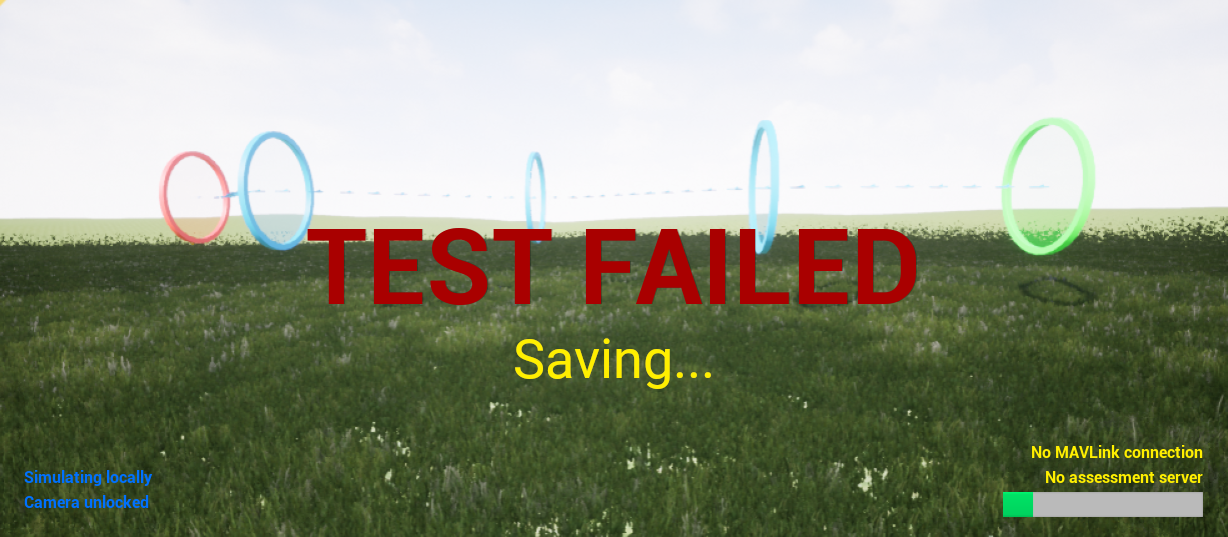
\includegraphics[width=\linewidth]{gui-2d.png}
    \caption{Interfejs graficzny wyświetlany na ekranie komputera}
    \label{fig:gui-2d}
\end{figure}

\begin{figure}[!h]
    \centering 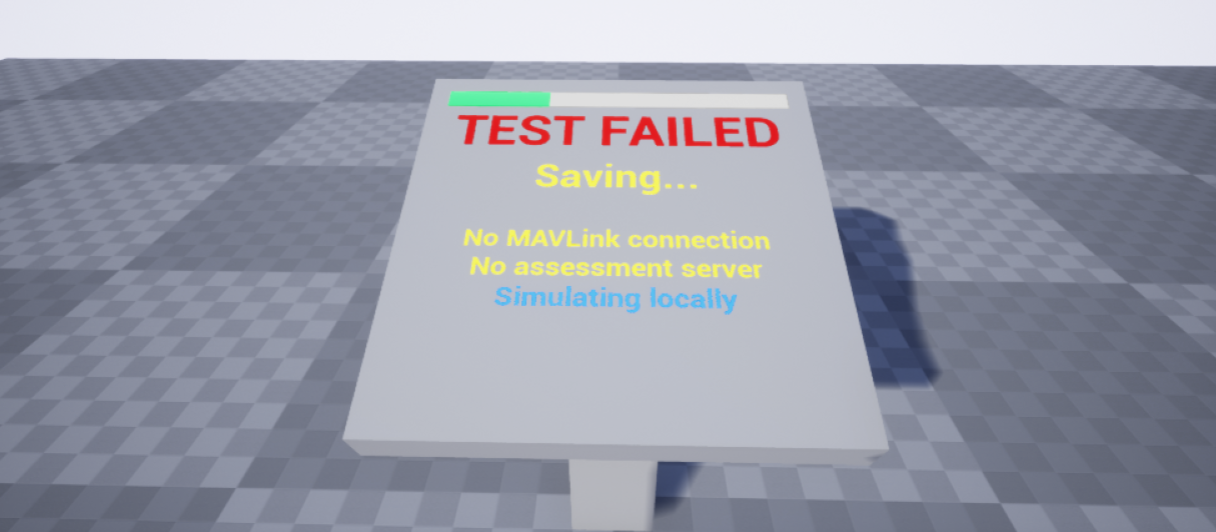
\includegraphics[width=\linewidth]{gui-vr.png}
    \caption{Interfejs graficzny w środowisku wirtualnej rzeczywistości}
    \label{fig:gui-vr}
\end{figure}

\begin{todo}
    źródła zastosowanych modeli i tekstur: własne, Raczek od Melavio, Igor Samek, Starter Content
\end{todo}

\subsection{Serwer oceny}
W przeciwieństwie do informacji o stanie BSP, dane na potrzeby oceny operatora nie muszą być dostarczone z najmniejszym możliwym opóźnieniem, natomiast dużo ważniejsza jest pewność dostarczenia kompletu pakietów. Z tego powodu do komunikacji z procesem oceniającym jakość pilotażu operatora, zastosowano protokół TCP/IP. Podczas rozwoju systemu, zauważono że wizualizacja jest znacznie częściej uruchamiana i zatrzymywana, więc przyjęto konwencję że program oceniający jest serwerem, a aplikacja wizualna łączącym się z nim klientem.

Jak wspomniano powyżej w rozdziale \ref{sec:architektura}, kluczową cechą serwera oceny jest łatwość pisania własnych funkcji oceniających. Aby ułatwić obsługę przesyłanych wiadomości dla przyszłych użytkowników, dane wewnątrz pakietów TCP przesyłane są w formie tekstowej, w formacie JSON\cite{json2017}. Taka reprezentacja danych jest czytelna dla człowieka, a zastosowane nazwy sprawiają że można ją zrozumieć bez czytania zewnętrznej dokumentacji. Aby systematycznie i szczegółowo opisać format wiadomości, przygotowano specyfikację JSON Schema\cite{jsonschema2020}. To rozwiązanie umożliwia automatyczną walidację wiadomości przez komunikujące się programy, ale też przez odpowiedni edytor tekstu. Przykład automatycznego wskazywania błędów oraz wyświetlania objaśnień przez edytor został przedstawiony na rysunku \ref{fig:schema-vscode}.

\begin{figure}[!h]
    \centering 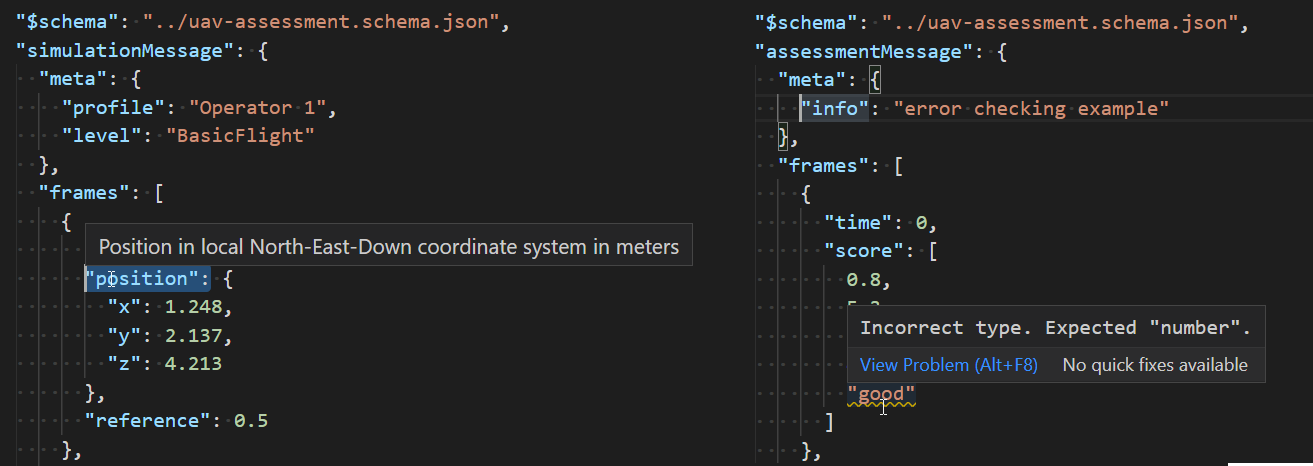
\includegraphics[width=\linewidth]{schema-vscode.png}
    \caption{Przykład dokumentacji i poprawy błędów wiadomości JSON w edytorze VS Code}
    \label{fig:schema-vscode}
\end{figure}

Zestaw informacji dostępnych do oceny opratora można odczytać ze specyfikacji formatu, w obiekcie \emph{simulationMessage}. W każdej wiadomości z danymi wysyłana jest nazwa profilu operatora, nazwa obecnie wykonywanego ćwiczenia oraz dodatkowy tekst informacyjny. Oprócz tego w polu \emph{frames} przesyłana jest lista ,,klatek'' symulacji, które odpowiadają klatkom obrazu rysowanym na ekranie. Każda klatka zawiera następujące informacje:

\begin{itemize}
    \item czas od rozpoczęcia podejścia [s]
    \item położenie w lokalnym układzie współrzędnych [m]
    \item prędkość w lokalnym układzie współrzędnych $ \left[ \frac{\text{m}}{\text{s}} \right] $
    \item kąty orientacji przestrzennej [°]
    \item odległość od trasy wzorcowej [m]
    \item odległość od najbliższej przeszkody [m]
    \item zdarzenia w formie listy tekstowych identyfikatorów
\end{itemize}

Poprawnie działający serwer oceny powinien na każdą otrzymaną wiadomość o stanie symulacji odpowiedzieć wiadomością z oceną w formacie \emph{assessmentMessage}. W każdej wiadomości wysyłany jest tekst informacyjny, który może zawierać na przykład nazwę wykorzystanej funkcji oceniającej, a także lista klatek oceny. Każdej klatce stanu symulacji powinna odpowiadać dokładnie jedna klatka oceny posiadająca taki sam znacznik czasu. Oprócz znacznika czasu, klatka oceny zawiera wynik oceny w postaci zbioru list rzeczywistych w ustalonej kolejności. Pierwszy element jest obowiązkowy, musi należeć do przedziału $ \langle 0; 1 \rangle $ i reprezentować ogólną jakość sterowania w danej chwili, przy czym wyższe wartości reprezentują lepsze sterowanie. Po otrzymaniu ta informacja zwrotna jest prezentowana operatorowi w trakcie wykonywania ćwiczenia, na rysunkach \ref{fig:gui-2d} oraz \ref{fig:gui-vr} jako prostokąt o zmiennym zielonym wypełnieniu. Kolejne wyniki oceny mogą zawierać dowolne wartości rzeczywiste, a ich znaczenie zależy od zastosowanej funkcji oceny. Aby móc je poprawnie interpretować ważne jest aby ich znaczenie lub przynajmniej zastosowana funkcja zostały przesłane w tekście informacyjnym, dzięki czemu będą zapisane do wynikowych plików CSV razem z wartościami oceny.

\subsection{Dokumentacja}
Aby ułatwić wykorzystanie systemu do własnych badań, przygotowano dokumentację dla użytkownika. Aktualna wersja jest publicznie dostępna w formie strony internetowej\cite{uavdocs2021}, obecnie jedynie w języku angielskim. Została podzielona na część podstawową \emph{User Guide} oraz zaawansowaną \emph{Developer Guide}. Zawiera listę niezbędnego oprogramowania, instrukcje jak pobrać kod źródłowy systemu oraz jak uruchomić i obsługiwać poszczególne aplikacje składowe. Opisano także sposób dodawania nowych ćwiczeń, modeli BSP, własnych funkcji oceniających i wprowadzania innych modyfikacji do działania systemu.

\begin{figure}[!h]
    \centering 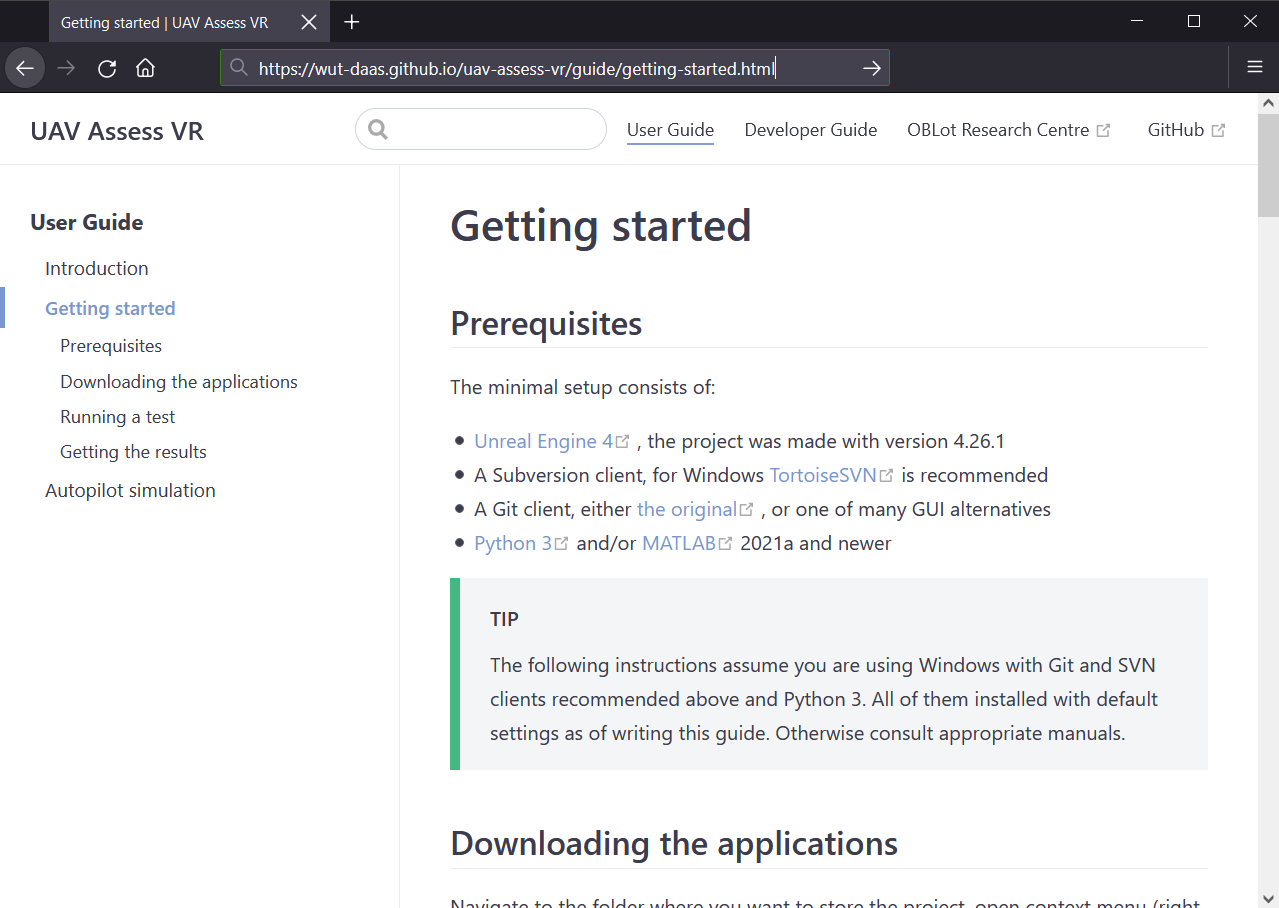
\includegraphics[width=0.8\linewidth]{dokumentacja-getting-started.png}
    \caption{Przykład strony z dokumentacji podstawowej}
    \label{fig:dokumentacja-getting-started}
\end{figure}

Treść dokumentacji jest opracowana w formie plików tekstowych formatu Markdown\cite{rfc7763}. Jedną z zalet takiego rozwiązania jest niezależność od używanego środowiska - systemu operacyjnego, edytora tekstu itp. Oprócz tego format jest bardzo popularny do opisu oprogramowania w formie plików \emph{README.md} umieszczonych w repozytoriach Git, dzięki czemu jest duża szansa że będzie znajomy dla użytkowników. Przykład demonstrujący tekst źródłowy m.~in. dla nagłówków, obrazów oraz treści komend wpisywanych do tekstowego terminala jest widoczny na rysunku \ref{fig:markdown}.

\begin{figure}[!h]
    \centering 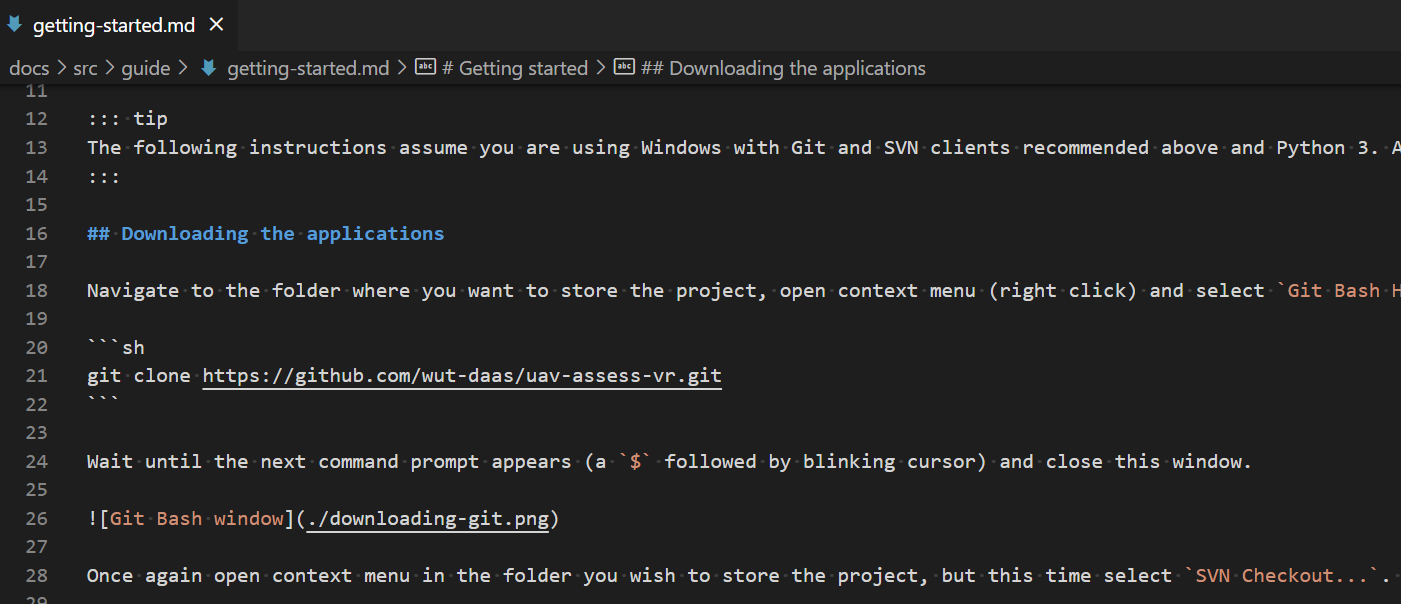
\includegraphics[width=\linewidth]{markdown.png}
    \caption{Fragment pliku źródłowego Markdown dokumentacji użytkownika}
    \label{fig:markdown}
\end{figure}

Każdy może zaproponować swoje poprawki do dokumentacji korzystając z mechanizmu \emph{Pull Request} oferowanego na platformie GitHub\cite{soft:github}. Ten termin można przetłumaczyć jako ,,prośba o włączenie do repozytorium'', i jest powszechnie stosowany w środowisku wolnego oprogramowania. Zaproponowane w ten sposób zmiany mogą być zaakceptowane przez administratora repozytorium, w tym przypadku przez członka zespołu Zakładu Automatyki i Osprzętu Lotniczego. Po akceptacji, pliki Markdown są przetwarzane na strony internetowe przez bibliotekę VuePress\cite{soft:vuepress}, a następnie automatycznie publikowane pod podanym adresem. Cały opisany proces odbywa się automatycznie na zewnętrznych serwerach, dzięki czemu użytkownicy mogą dalej poprawiać dokumentację po zakończeniu pracy oryginalnego autora.
